This section will be explained through an example where the input is the color corrected image of Figure \ref{fig:faceMasks}\textit{a}.



In short, initially is the input image padded with zeros on all sides by a $4x4$ kernel in order for future morphological operations to work as intended. Then are several masks derived that are used for image segmentation in order to narrow the search space for eyes and mouth. To be clear, we will call the mask that marks out where the estimated face is in the image for \textit{face mask} and the result of this phase for \textit{output}. The output is essentially an image derived from a narrowed face mask in form of a rectangle that precisely covers the eyes and mouth, see Figure \ref{fig:rotationAndOutput}\textit{c} for an example. When the face mask is found we can search for the eyes and mouth. The eyes and mouth will then be used to compute the output. 

\begin{figure}[H]
\centering

\begin{subfigure}{.4\textwidth}
  \centering
  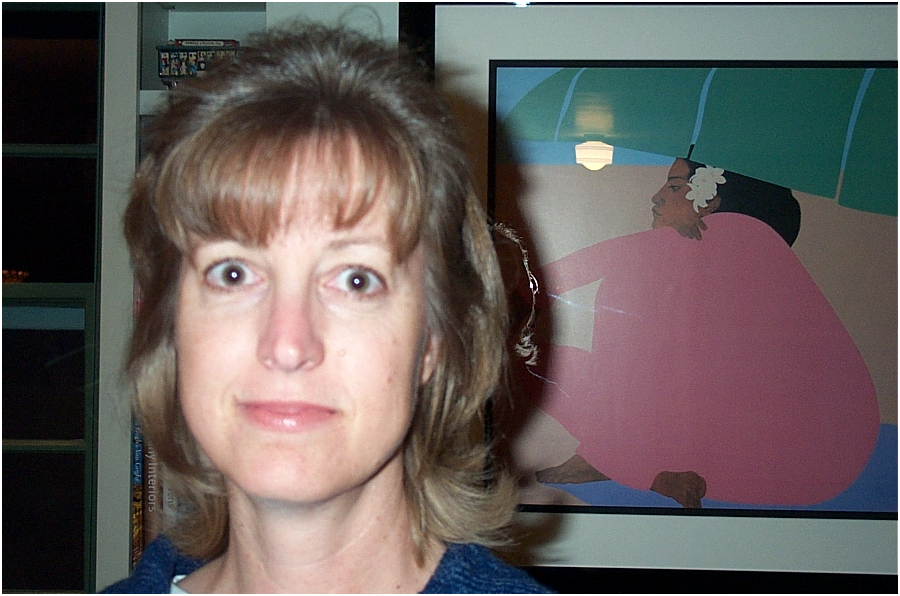
\includegraphics[width=0.95\textwidth]{img/fd/Original.png}
  \caption{}
  % \label{fig:sub1}
\end{subfigure}%

\begin{subfigure}{.24\textwidth}
  \centering
  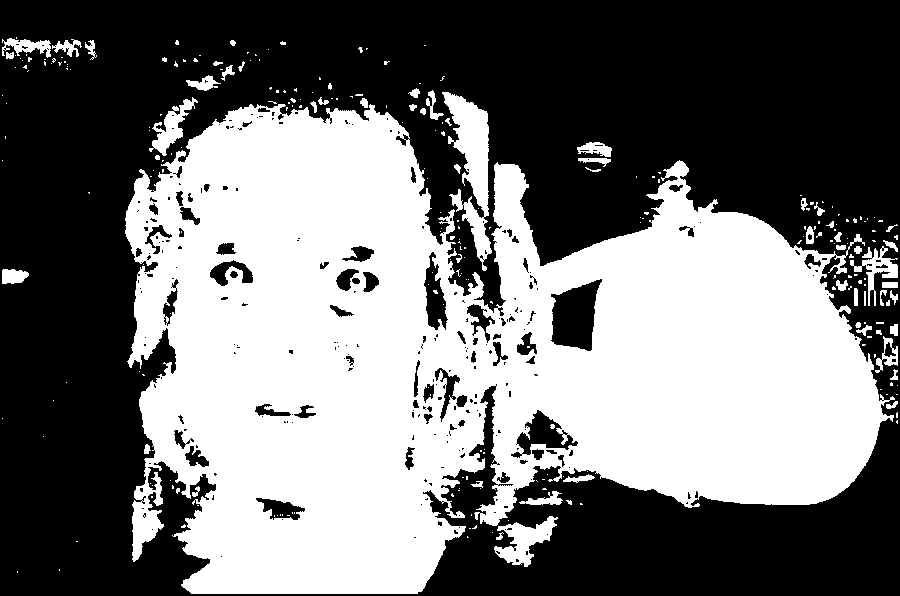
\includegraphics[width=0.95\textwidth]{img/fd/EstimatedSkinMask.png}
  \caption{}
  % \label{fig:sub1}
\end{subfigure}%
\begin{subfigure}{.24\textwidth}
  \centering
  % 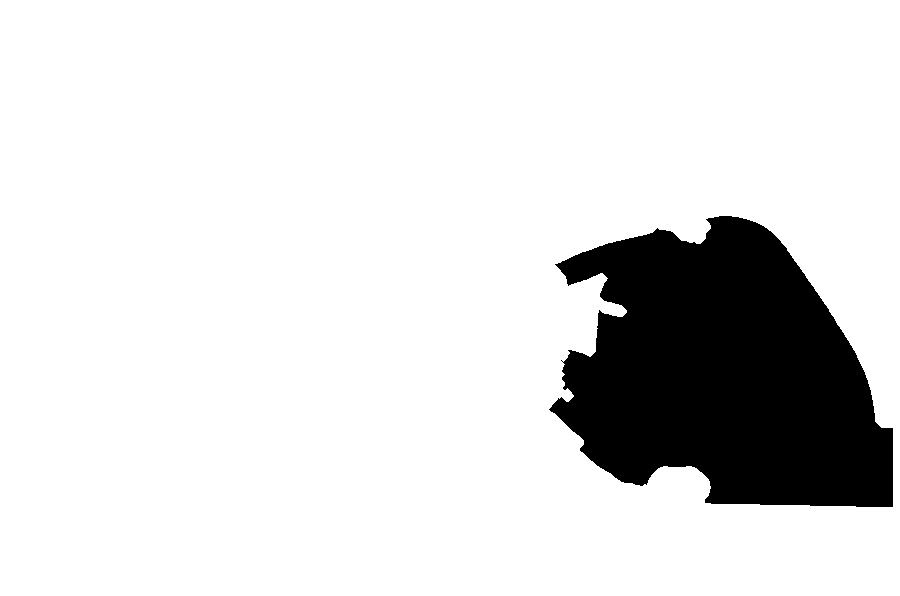
\includegraphics[width=0.95\textwidth]{img/fd/ForeGroundMask.png}
  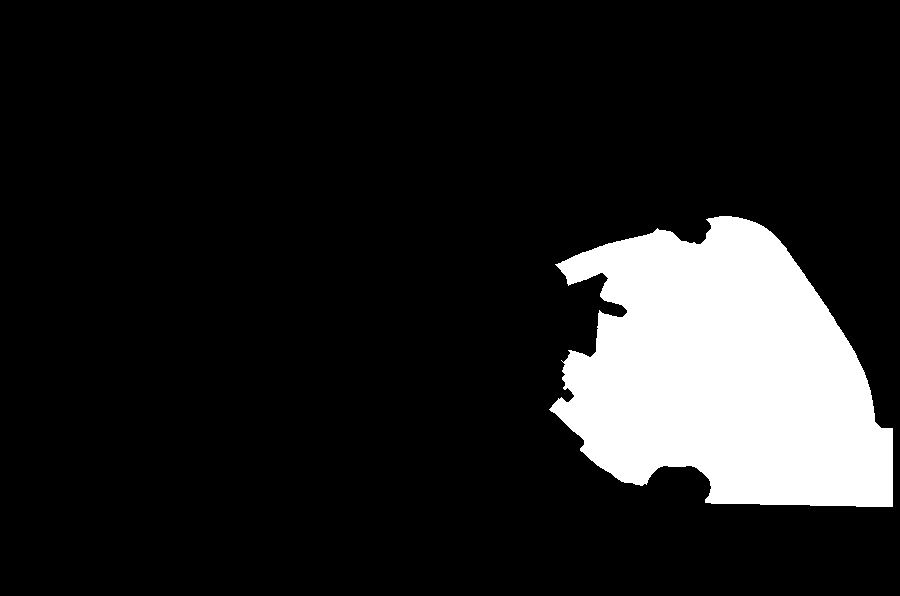
\includegraphics[width=0.95\textwidth]{img/fd2/BackgroundMask.png}
  \caption{}
  % \label{fig:sub2}
\end{subfigure}
\begin{subfigure}{.24\textwidth}
  \centering
  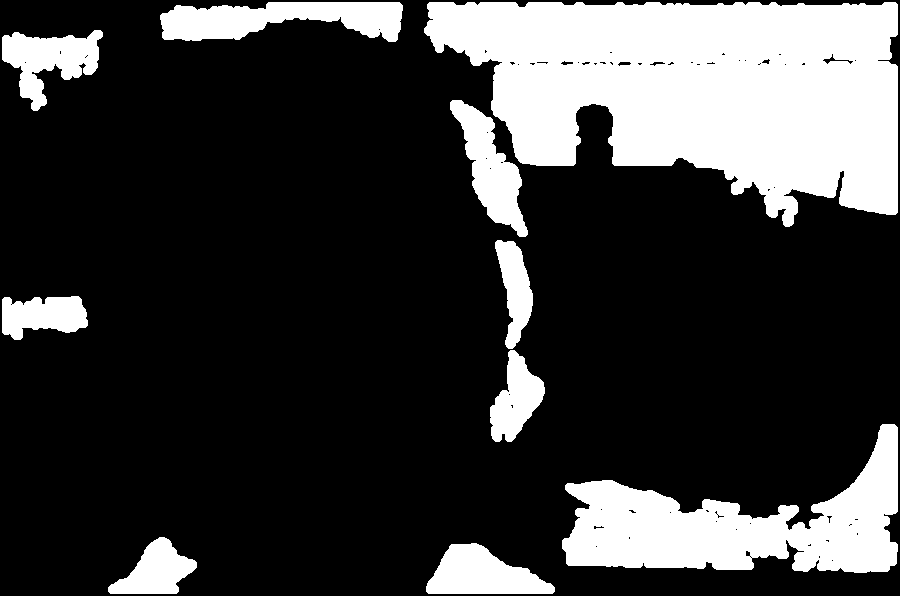
\includegraphics[width=0.95\textwidth]{img/fd/NonFaceMask.png}
  \caption{}
  % \label{fig:sub2}
\end{subfigure}
\begin{subfigure}{.24\textwidth}
  \centering
  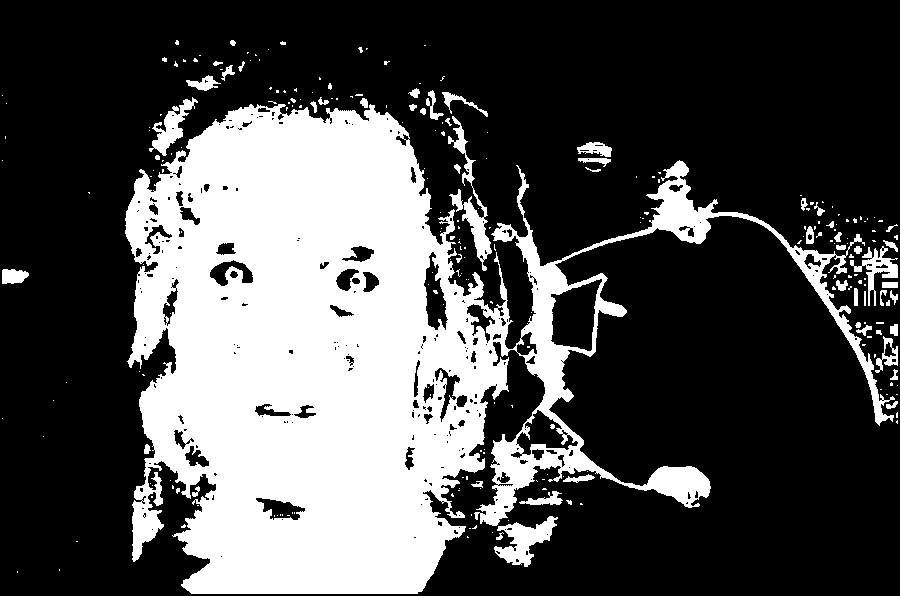
\includegraphics[width=0.95\textwidth]{img/fd/ForegroundMaskAndEstimatedSkinMaskAndNonFaceMask.png}
  \caption{}
  % \label{fig:sub2}
\end{subfigure}


\begin{subfigure}{.24\textwidth}
  \centering
  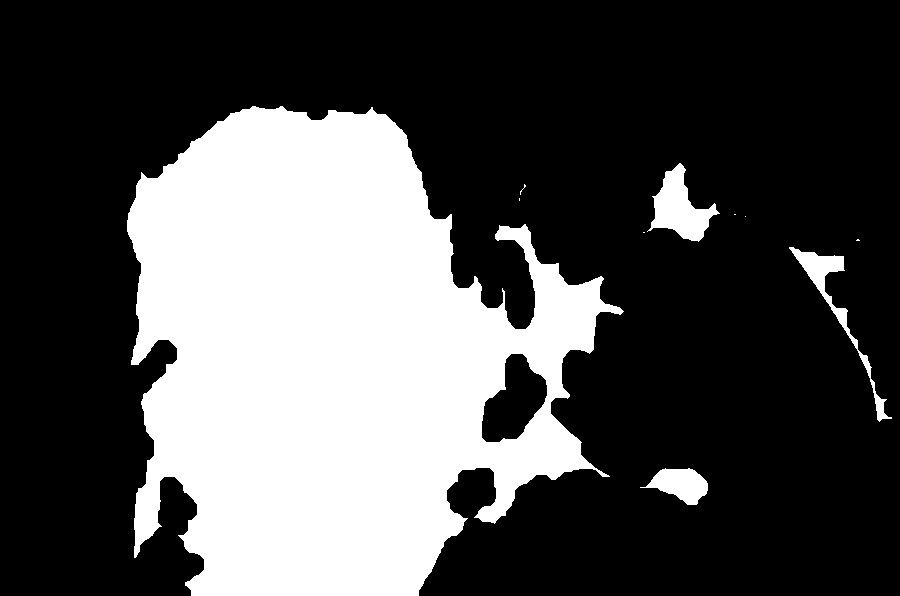
\includegraphics[width=0.95\textwidth]{img/fd/ClosingOnFaceMask.png}
  \caption{}
  % \label{fig:sub2}
\end{subfigure}
\begin{subfigure}{.24\textwidth}
  \centering
  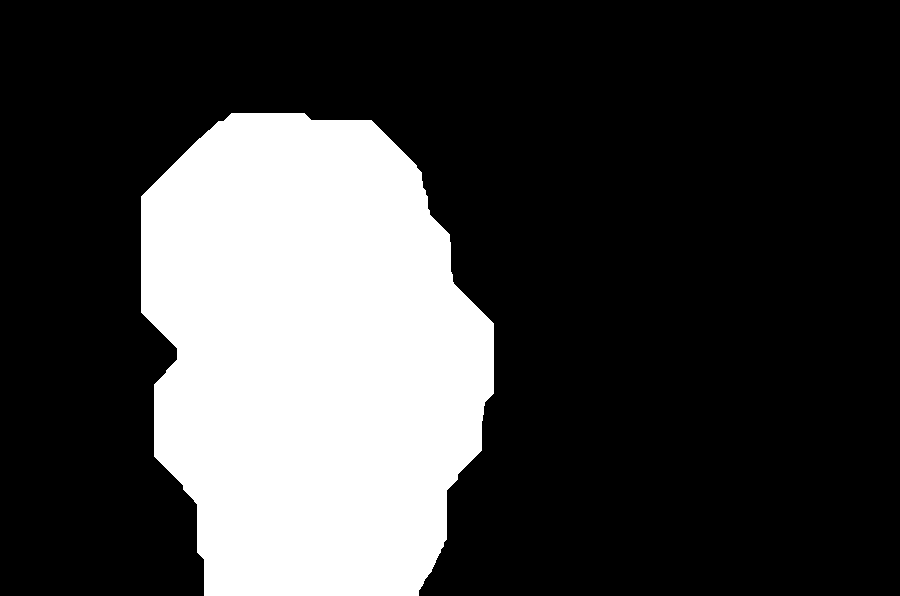
\includegraphics[width=0.95\textwidth]{img/fd/ShrinkFaceMask.png}
  \caption{}
  % \label{fig:sub2}
\end{subfigure}
\begin{subfigure}{.24\textwidth}
  \centering
  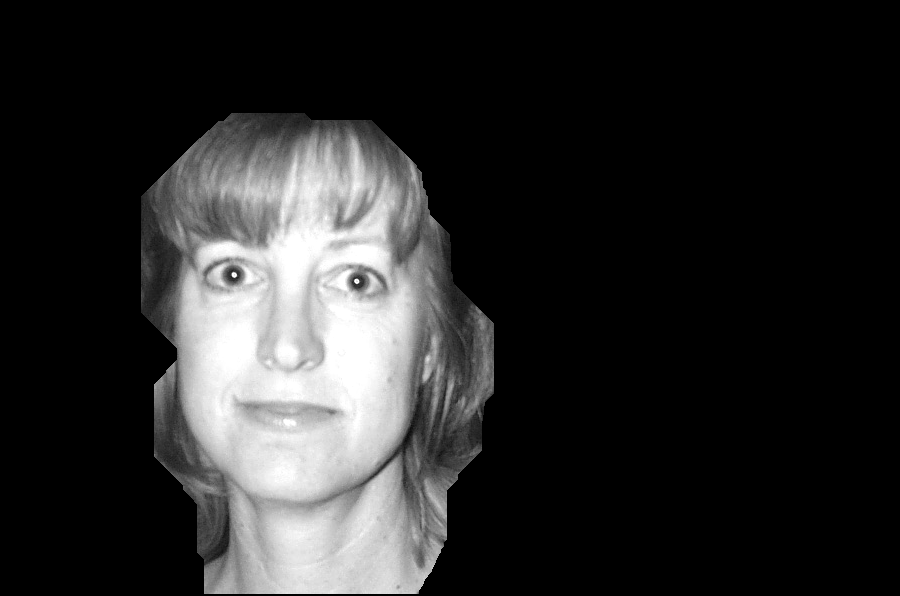
\includegraphics[width=0.95\textwidth]{img/fd/ImadjustGrayFace.png}
  \caption{}
  % \label{fig:sub2}
\end{subfigure}
\begin{subfigure}{.24\textwidth}
  \centering
  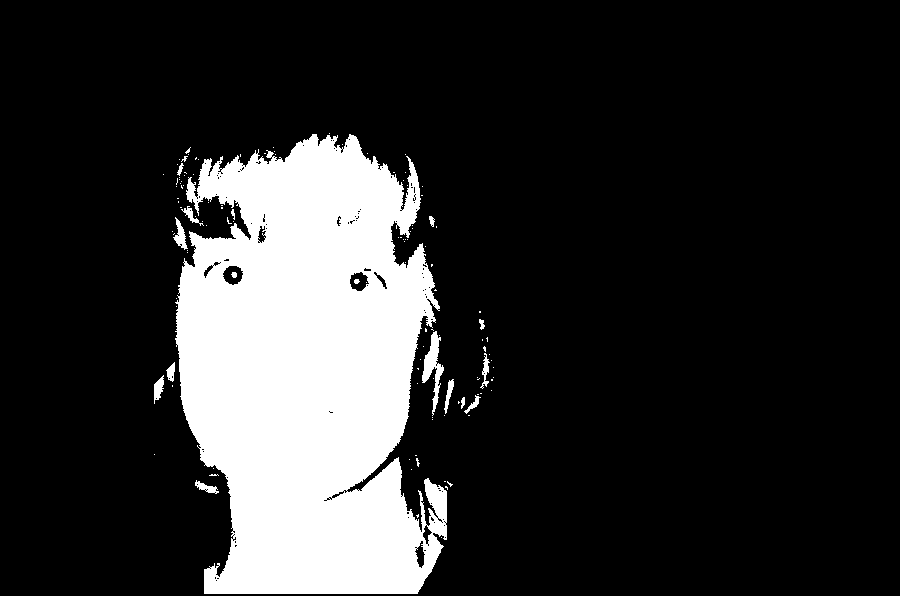
\includegraphics[width=0.95\textwidth]{img/fd/ThresholdGrayFace.png}
  \caption{}
  % \label{fig:sub2}
\end{subfigure}
\begin{subfigure}{.24\textwidth}
  \centering
  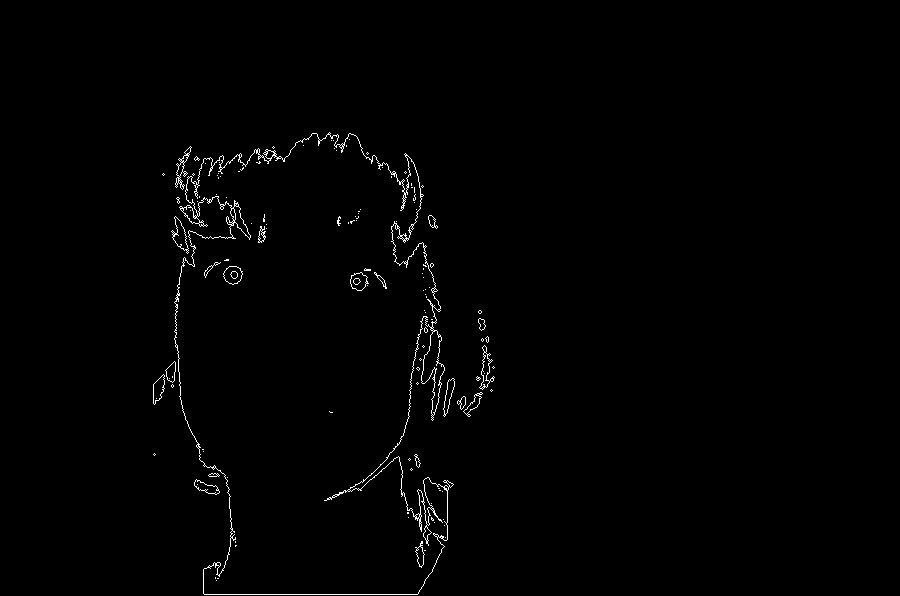
\includegraphics[width=0.95\textwidth]{img/fd/FilteredFaceMask.png}
  \caption{}
  % \label{fig:sub2}
\end{subfigure}
% \begin{subfigure}{.24\textwidth}
%   \centering
%   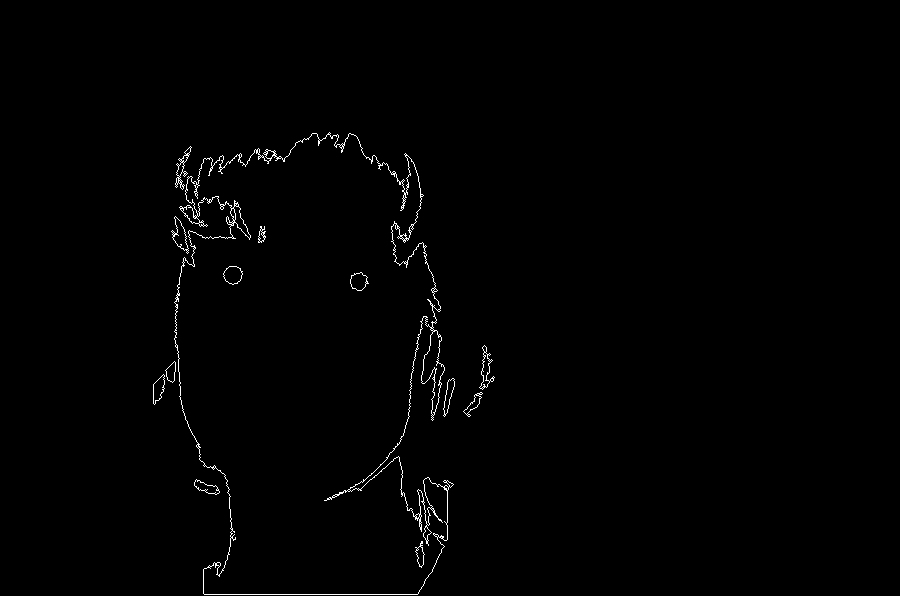
\includegraphics[width=0.95\textwidth]{img/fd/FilteredFaceMask2.png}
%   \caption{}
%   % \label{fig:sub2}
% \end{subfigure}
% \begin{subfigure}{.24\textwidth}
%   \centering
%   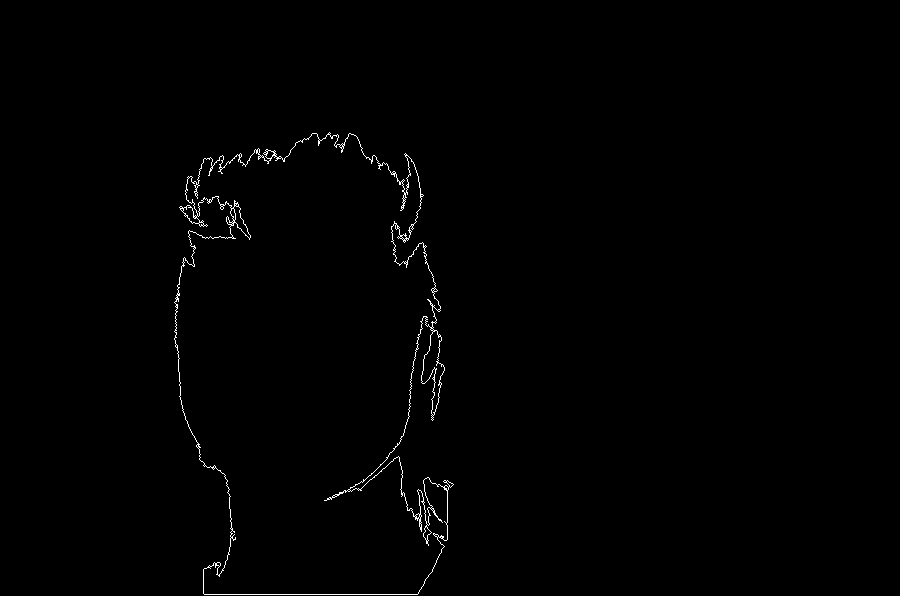
\includegraphics[width=0.95\textwidth]{img/fd/FilteredFaceMask3.png}
%   \caption{}
%   % \label{fig:sub2}
% \end{subfigure}
\begin{subfigure}{.24\textwidth}
  \centering
  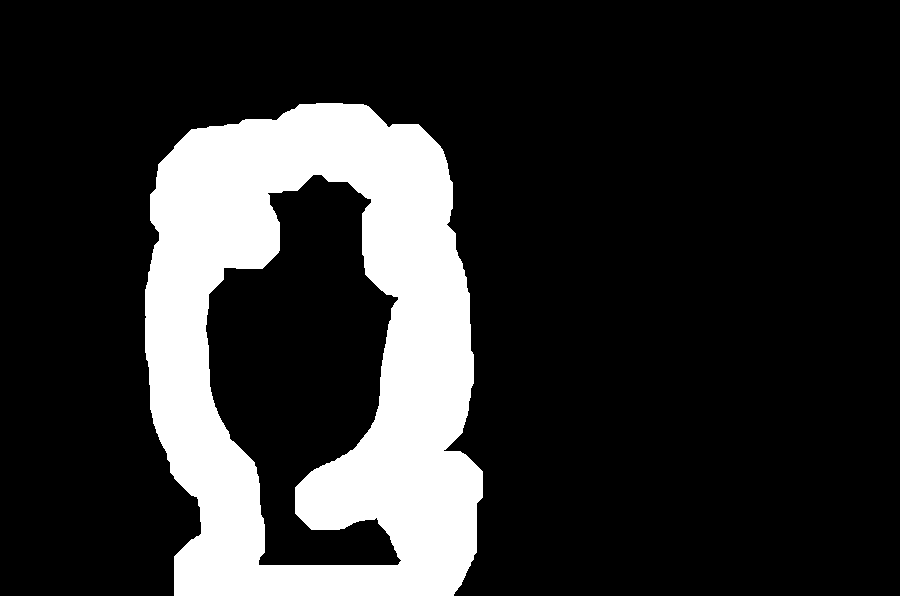
\includegraphics[width=0.95\textwidth]{img/fd/FilteredFaceMask4.png}
  \caption{}
  % \label{fig:sub2}
\end{subfigure}
\begin{subfigure}{.24\textwidth}
  \centering
  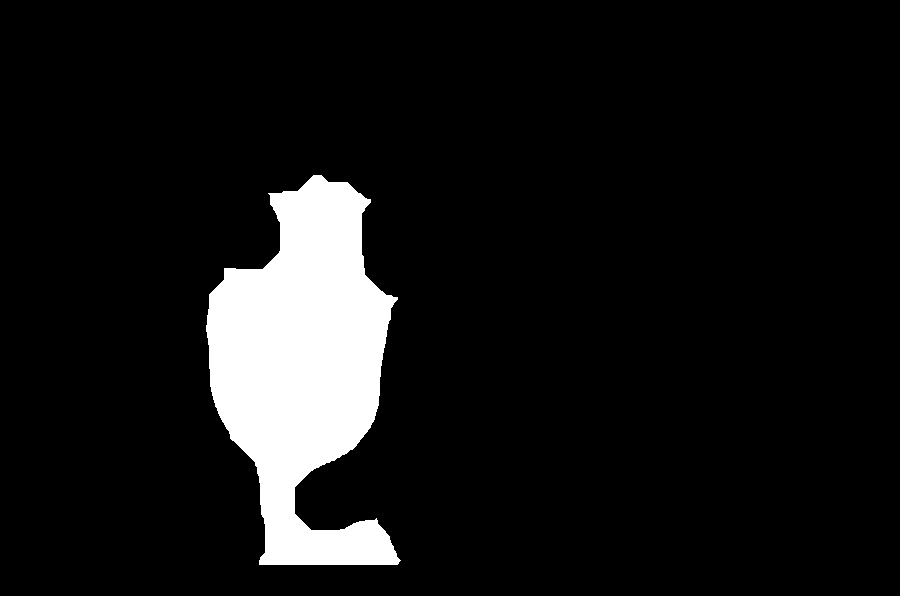
\includegraphics[width=0.95\textwidth]{img/fd/FilteredFaceMask5.png}
  \caption{}
  % \label{fig:sub2}
\end{subfigure}
% \begin{subfigure}{.24\textwidth}
%   \centering
%   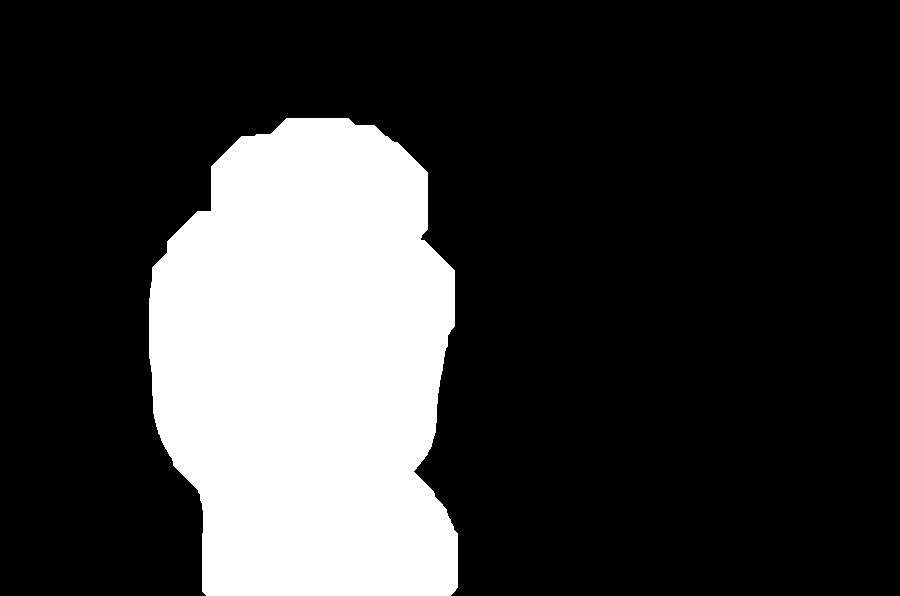
\includegraphics[width=0.95\textwidth]{img/fd/FilteredFaceMask6.png}
%   \caption{}
%   % \label{fig:sub2}
% \end{subfigure}
\begin{subfigure}{.24\textwidth}
  \centering
  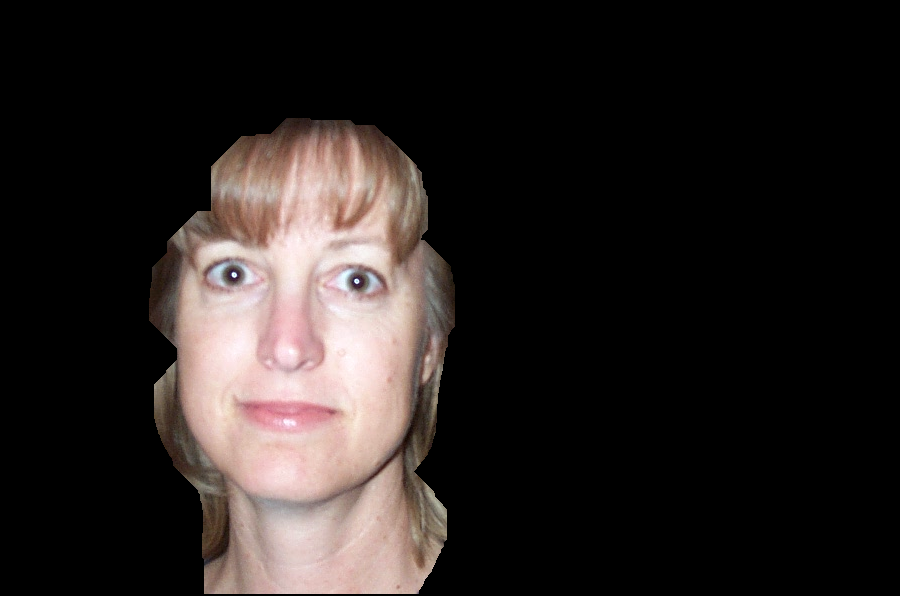
\includegraphics[width=0.95\textwidth]{img/fd/FilteredFaceMask6_Face.png}
  \caption{}
  % \label{fig:sub2}
\end{subfigure}

\caption{Masks \textit{(b-l)} that are generated during the process of deriving the final face \textit{m} from input image \textit{a}.}
\label{fig:faceMasks}
\end{figure}


\subsubsection{Estimated skin mask}
After padding the color corrected input image several masks are computed. At first is a mask for estimated skin regions computed through thresholding inside the \textit{YCbCr} color space. See Equation \ref{eq:estimatedSkinMask} for the specific values we use and Figure \ref{fig:faceMasks}\textit{b} for the estimated skin mask of this example.

\begin{equation} \label{eq:estimatedSkinMask}
\begin{split}
estimatedSkinMask = and( & and(C_{b}> 95, \ C_{b} < 145), \\
 & and(C_{r} > 132, \ C_{r} < 165))
\end{split}
\end{equation}

\subsubsection{Background mask}
Next follows the computation of a mask for the background (Figure \ref{fig:faceMasks}\textit{c}), or in more particular, a mask containing large homogeneous regions of low frequency. This as we assume that a face contains a lot of high frequency parts while background regions, e.g. walls, often are homogeneous. To avoid that small regions in the face are selected for this mask we remove all regions with areas containing less than $5$ percent of the pixels of the image.

The function takes the gray version of the input image as argument. Furthermore, we first increase the contrast of the image by using \textit{Matlab's} \textit{imadjust} function. Then we use edge filtering on the image with the \textit{Canny} kernel. This will highlight the edges of the image. We then perform some morphological operations that will implicitly threshold the image and deliver a binary mask containing blobs that represent each region, see Figure \ref{fig:AllBackgroundBlobs}. As previously mentioned before continuing any computation, we remove small blobs.

\begin{figure}[H]
\centering
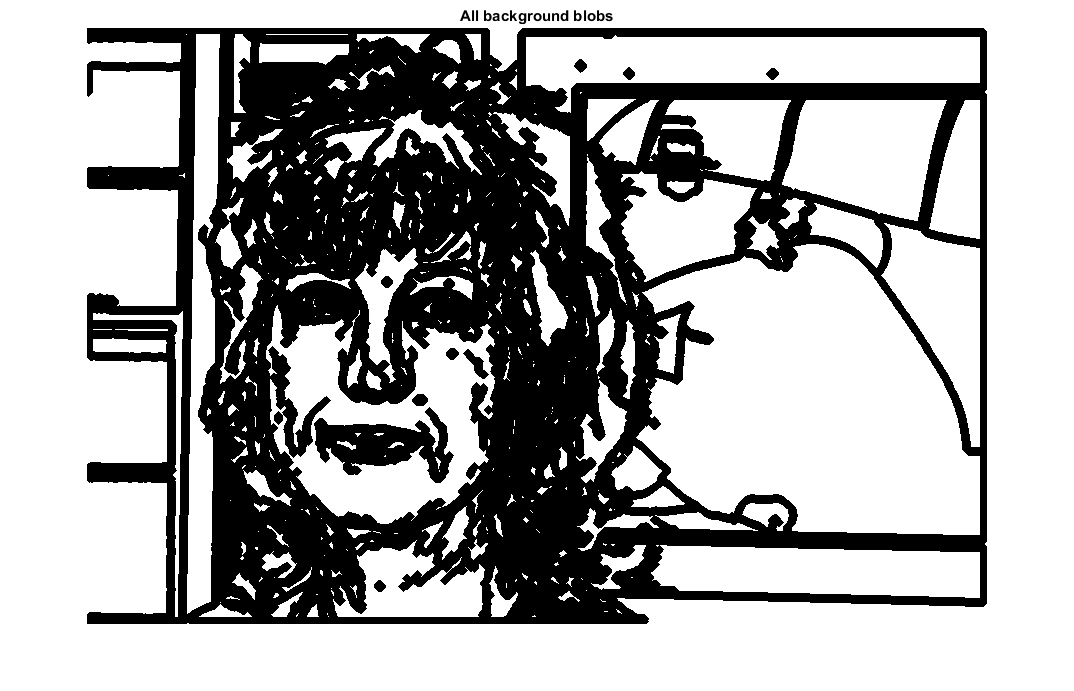
\includegraphics[width=0.4\textwidth]{img/fd2/AllBackgroundBlobs.png}
\caption{Segmented image for determining the background mask.}
\label{fig:AllBackgroundBlobs}
\end{figure}



Then we derive a gray scale image representing the amount of high frequencies in each region by performing a median filtering of the input image followed by a filtering with the \textit{Laplacian of Gaussian} kernel. The median filter will remove unwanted noise as we are only interested in those frequencies caused by the actual objects in our image. The LoG filter will first smooth the image a bit more by the Gaussian kernel before the Laplacian kernel is applied in order to give us the more important frequencies of the image. Given this computed image containing the high frequency information we can for each region blob calculate the percentage of high frequency. We conclude that if the high frequency part is less than $0.8$ percent, it is likely that this region of the image is part of the background and that we therefore can add this blob to the background mask.

\subsubsection{Non face regions mask}
Next follows the computation of a mask containing regions of the image that we deem will not be part of the face, see Figure \ref{fig:faceMasks}\textit{d}. This through the utilization of the YCbCr as well as the HSV color space, as seen in Equation \ref{eq:nonFaceMask}. The mask is before being used also subject of some morphological operations (opening and removal of small blobs), this in order to remove small parts, like eyes, which sometimes are included in this mask.

\begin{equation} \label{eq:nonFaceMask}
\begin{split}
  nonSkinMask1 & = C_{b} > C_{r} + 10 \\
  nonSkinMask2 & = V < S - 0.2 \\
  nonFaceMask & = or(nonSkinMask1, \ nonSkinMask2)
\end{split}
\end{equation}

\subsubsection{Face mask}
Now we can combine the estimated skin mask (Figure \ref{fig:faceMasks}\textit{b}) with the background mask (Figure \ref{fig:faceMasks}\textit{c}) as well as the mask containing non face regions (Figure \ref{fig:faceMasks}\textit{d}) in order to derive our first estimation for the face mask (Figure \ref{fig:faceMasks}\textit{e}). Worth noticing is that Figure \ref{fig:faceMasks}\textit{e} both contains large parts of the woman's face as well as parts of the pictured person's face in the background painting. The combining is essentially done by an AND operation; \\ 
\-\hspace{1.0cm} \textit{AND(estimatedSkinMask, $\neg$ backgroundMask, $\neg$ nonFaceMask)}.

To improve this estimation we perform opening operations, this will give us Figure \ref{fig:faceMasks}\textit{f}. Then to further improve the estimation all the holes in the derived mask is filled before the largest blob is selected to be the new estimation. This new estimation will then be the subject of an iterative opening process that shrinks the mask as much as possible while making sure that there still is a blob left in the mask, see the result of this process in Figure \ref{fig:faceMasks}\textit{g}.

We now try to further improve the estimation while we in the process also try to derive eye candidate masks. To do this we first compute a gray image over the face, Figure \ref{fig:faceMasks}\textit{h}, by utilization of our face mask estimation. If the gray face image has one large bright part and one large dark part, which corresponds to the person being lit by a light from the side, and that the mean values of these regions are sufficiently diverse we brighten the dark part of the face by adding $80$ percent of the mean value difference to each pixel of the dark part. This reasoning is illustrated by Figure \ref{fig:grayFace} and notice that both eyes are represented among the eye candidates in Figure \ref{fig:grayFace}\textit{f} while only one eye is represented among the eye candidates in \ref{fig:grayFace}\textit{c}. Furthermore, to compute the bright and dark part of the image we use the Y component of the YCbCr color space. 

\begin{figure}[H]
\centering

\begin{subfigure}{.16\textwidth}
  \centering
  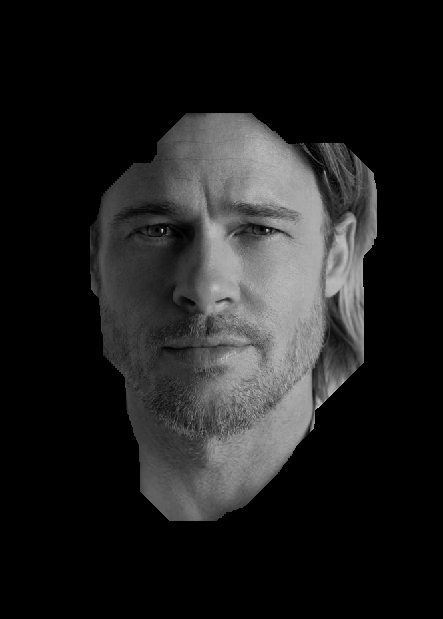
\includegraphics[width=0.95\textwidth]{img/fd3/grayFaceNormall.png}
  \caption{}
\end{subfigure}%
\begin{subfigure}{.16\textwidth}
  \centering
  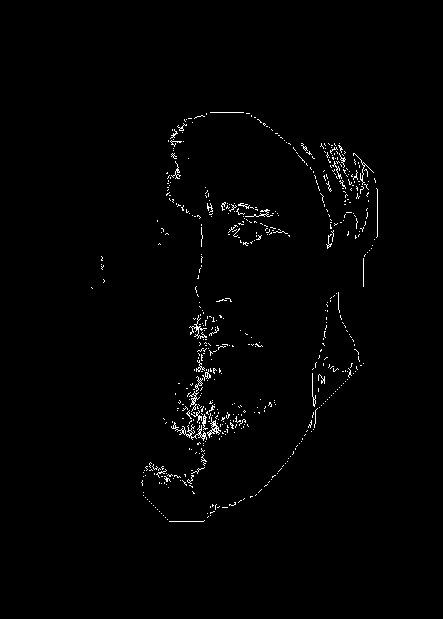
\includegraphics[width=0.95\textwidth]{img/fd3/grayFaceNormalFilteredFaceMask.png}
  \caption{}
\end{subfigure}%
\begin{subfigure}{.16\textwidth}
  \centering
  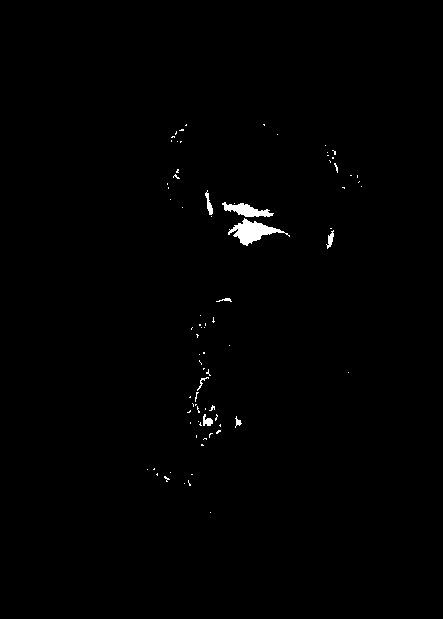
\includegraphics[width=0.95\textwidth]{img/fd3/grayFaceNormalEyeCandidates.png}
  \caption{}
\end{subfigure}%
\begin{subfigure}{.16\textwidth}
  \centering
  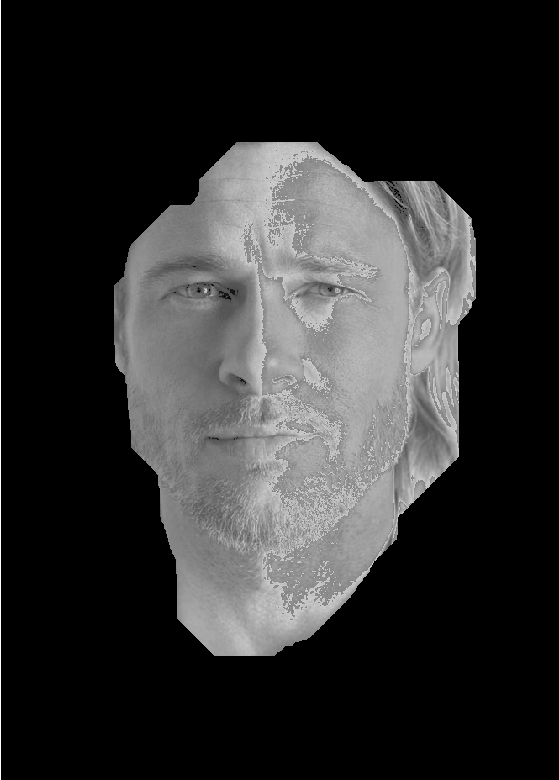
\includegraphics[width=0.95\textwidth]{img/fd3/grayFaceSpecial.png}
  \caption{}
\end{subfigure}%
\begin{subfigure}{.16\textwidth}
  \centering
  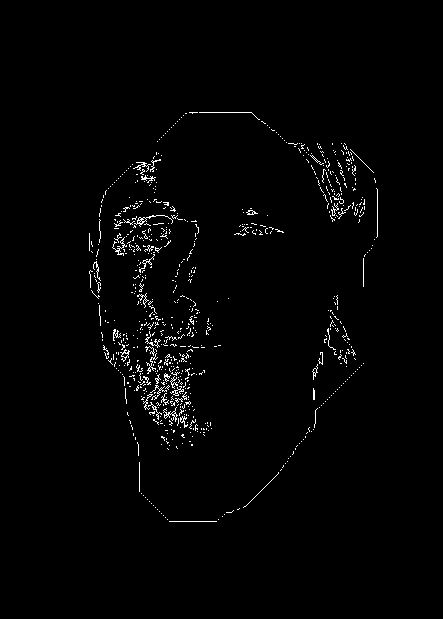
\includegraphics[width=0.95\textwidth]{img/fd3/grayFaceSpecialFilteredFaceMask.png}
  \caption{}
\end{subfigure}%
\begin{subfigure}{.16\textwidth}
  \centering
  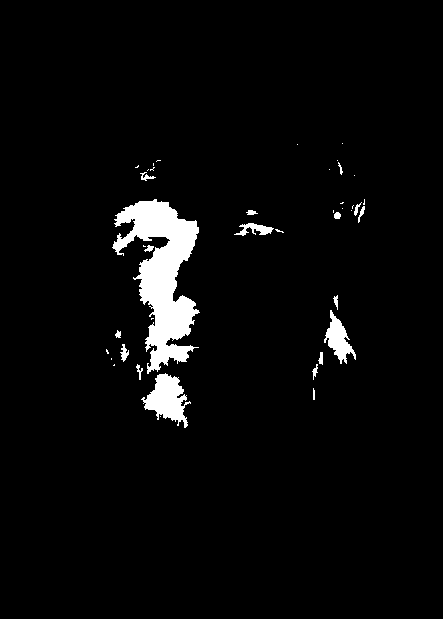
\includegraphics[width=0.95\textwidth]{img/fd3/grayFaceSpecialEyeCandidates.png}
  \caption{}
\end{subfigure}%

\caption{Referea i texten!}
\label{fig:grayFace}
\end{figure}

By thresholding the gray face image by $0.47$ we receive the binary image seen in Figure \ref{fig:faceMasks}\textit{i}. This binary image is only computed to be used for deriving the face contours, see Figure \ref{fig:faceMasks}\textit{j}. This is done by the unconventional way of using filtering with the Laplacian kernel, however through experimentation we have found out that this method works better for this specific case than other edge detection algorithms. This filtered face mask is then influenced by a number of morphological and binary operations. We first extract the main contour of the face, this is done by filling in all the holes and XOR-ing this mask with an eroded version of this mask. It is done in this particular way as if the face contour instead was selected by the blob with largest area, we could get a blob inside the face instead, e.g. a contour of someones beard. If we on the other hand would select the blob that has the largest convex hull the face border could sometimes be connected to the borders of the eyes (e.g. slight side pose), eliminating one of the eyes from our mask, which is not what we want. By selecting regions that lie inside of the face contour we can extract different masks for eye candidates, combined they make up \\ Figure \ref{fig:eyeMap}\textit{e}.

Now that we have computed our eye candidates that help us narrow the search space for the actual eyes, we can try to improve the estimated face mask even more. What led us to this idea is that it would be nice if we could get rid of excessive hair and the neck 
from some faces. For example, removing the neck will also remove eventual necklaces that could interfere with the process of finding the eyes. The same applies to hair, as curls often form circular patterns that could be mistaken for an eye.

We begin with dilating the contour of the face quite a lot. This as the hair line of our face contour often consist of a zig-zag pattern and that dilation will therefore smooth out these lines, see Figure \ref{fig:faceMasks}\textit{k}. Now by filling in the holes (because of this operation we padded the image with zeros in the beginning) and XOR-ing with the previous state we can derive Figure \ref{fig:faceMasks}\textit{l}. Notice how the neck in this case is almost in an own blob, this is what we wanted, but this did not happen with this particular image. If the neck would be separated in an own blob, we would select the largest blob to be our new estimation of the face mask. To determine the final face mask used to derive the face image in Figure \ref{fig:faceMasks}\textit{m} we only need to perform some iterative dilation to our estimation. Notice how we got rid of some of the hair and that we almost got rid of the neck in this case by comparing with Figure \ref{fig:faceMasks}\textit{h}.




\subsubsection{Eye map}

In order to deliver a precise output image we first need to locate the positions of the eyes and mouth. To extract the eyes we go by the method described in \cite{fdInColorImages} and explained in the theory section above. By Equation \ref{eq:eyeMapChroma} we compute the chromatic component of the eye map which can be seen in Figure \ref{fig:eyeMap}\textit{a}. More over is the luminance component of the eye map computed according to Equation \ref{eq:eyeMapLuma} and displayed in Figure \ref{fig:eyeMap}\textit{b} while the resulting original eye map is seen in Figure \ref{fig:eyeMap}\textit{c}.

\begin{figure}[H]
\centering

\begin{subfigure}{.33\textwidth}
  \centering
  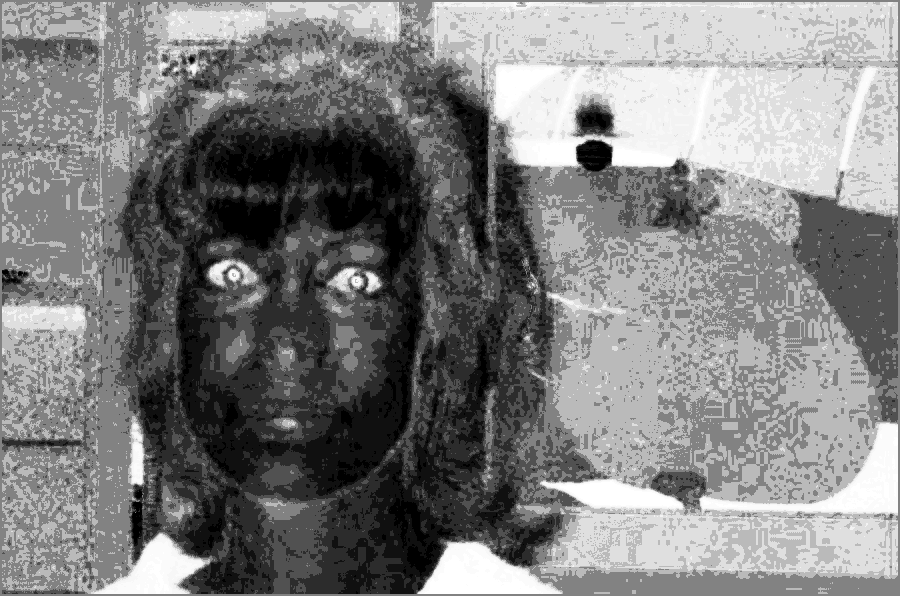
\includegraphics[width=0.95\textwidth]{img/fd2/EyeMapChroma.png}
  \caption{}
  % \label{fig:sub1}
\end{subfigure}%
\begin{subfigure}{.33\textwidth}
  \centering
  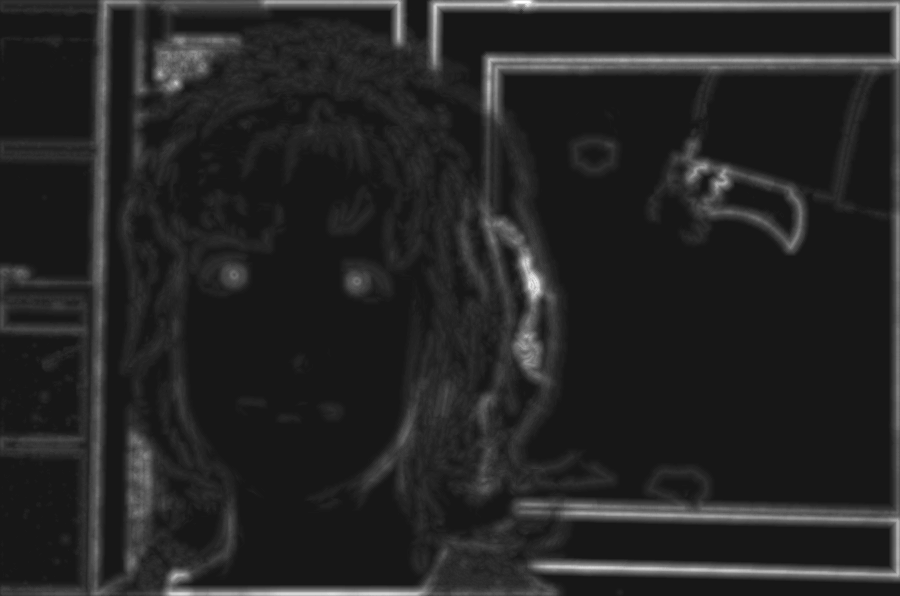
\includegraphics[width=0.95\textwidth]{img/fd2/EyeMapLuma.png}
  \caption{}
  % \label{fig:sub1}
\end{subfigure}%
\begin{subfigure}{.33\textwidth}
  \centering
  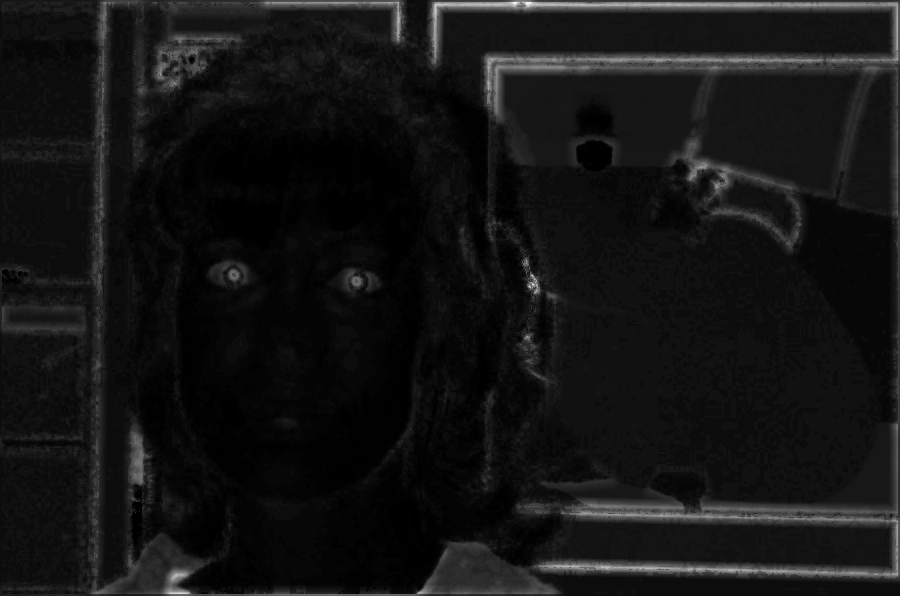
\includegraphics[width=0.95\textwidth]{img/fd/OriginalEyeMap.png}
  \caption{}
  % \label{fig:sub1}
\end{subfigure}%

\begin{subfigure}{.33\textwidth}
  \centering
  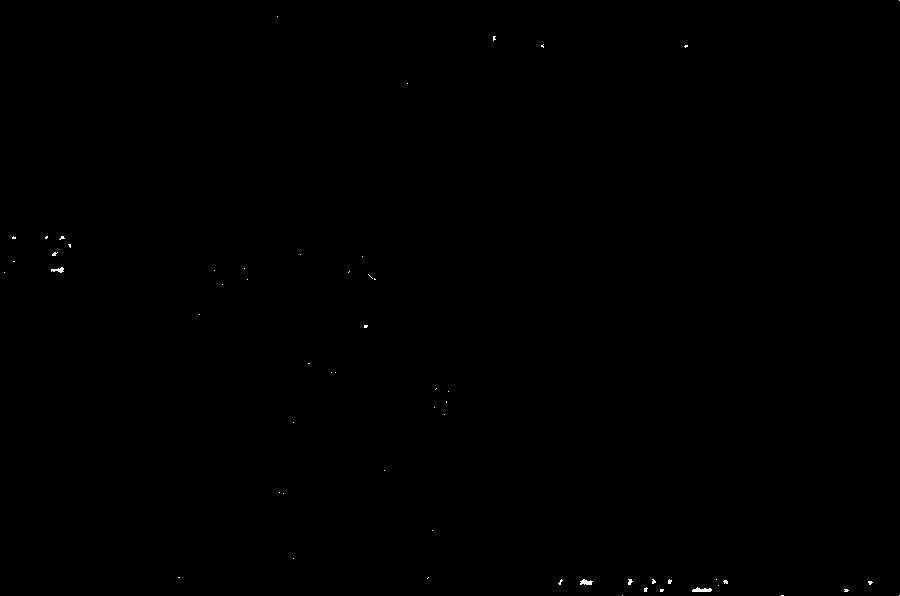
\includegraphics[width=0.95\textwidth]{img/fd/OverSaturatedMask.png}
  \caption{}
  % \label{fig:sub1}
\end{subfigure}%
\begin{subfigure}{.33\textwidth}
  \centering
  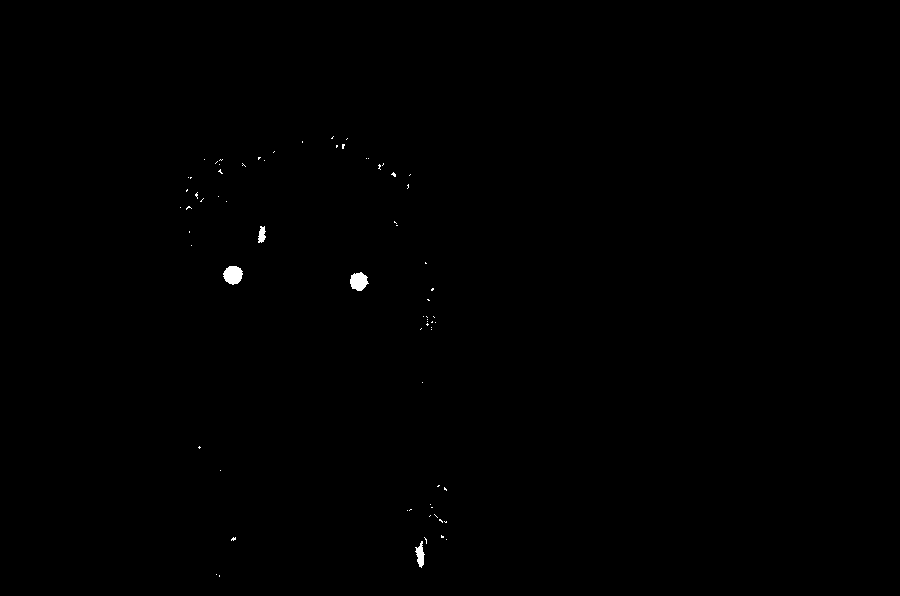
\includegraphics[width=0.95\textwidth]{img/fd/FilteredFaceMaskEyesReal.png}
  \caption{}
  % \label{fig:sub1}
\end{subfigure}%
\begin{subfigure}{.33\textwidth}
  \centering
  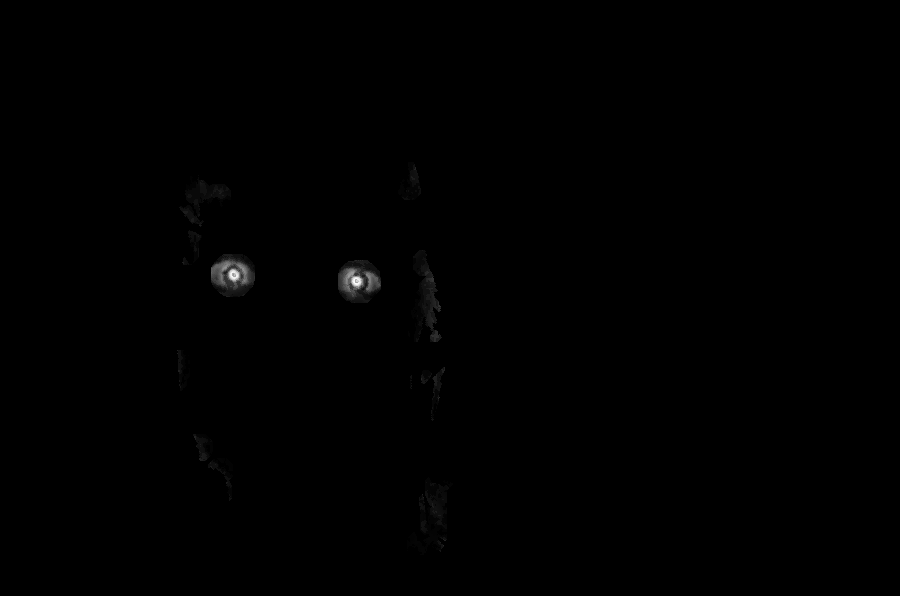
\includegraphics[width=0.95\textwidth]{img/fd/EyeMap2.png}
  \caption{}
  % \label{fig:sub1}
\end{subfigure}%

\caption{Process of computing the eyes' locations. (a) is the chromatic component of the eye map, (b) the luminance component, (c) the original eye map, (d) the mask of over saturated regions, (e) the eye candidates while (f) is the final eye map.}
\label{fig:eyeMap}
\end{figure}

To narrow the search space for the \textit{Hough transform} that will try to find bright circles in the eye map, we want to detract as much as possible from it while leaving the eyes present. Through experimental testing we have found that oversaturated parts of some images have an negative influence on the outcome of the Hough transform when it is searching for the locations of the eyes. Therefore we attempt to minify their footprint by the construction and utilization of a mask containing those regions. In this particular image there are no prominent oversaturated regions as is easily understood by viewing the oversaturated mask in Figure \ref{fig:eyeMap}\textit{d}. However Figure \ref{fig:overSaturated} illustrates that there indeed is oversaturated parts of some images and that the oversaturation usually avoid the eye regions which let us detract this mask from the original eye map. 


\begin{figure}[H]
\centering

\begin{subfigure}{.33\textwidth}
  \centering
  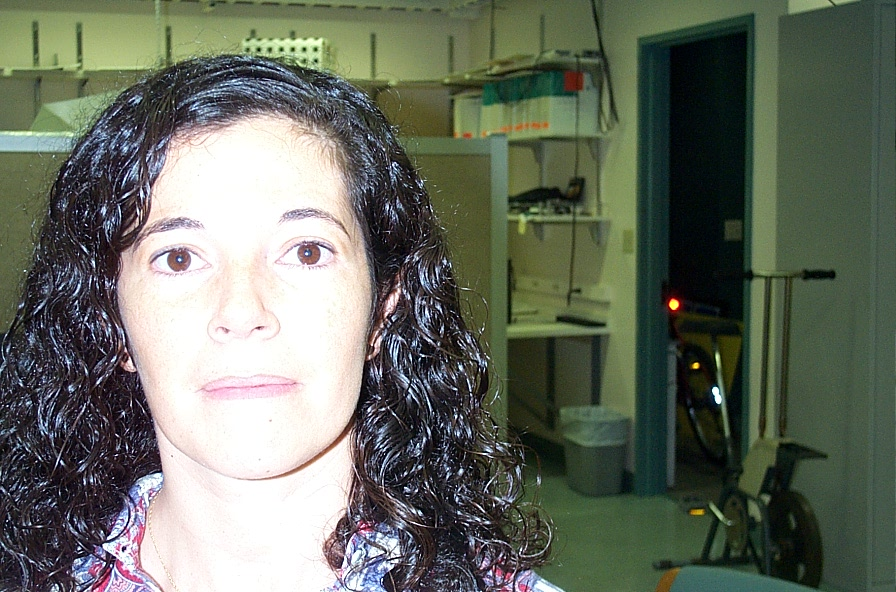
\includegraphics[width=0.95\textwidth]{img/fd2/overSaturated_input.jpg}
  \caption{}
\end{subfigure}%
\begin{subfigure}{.33\textwidth}
  \centering
  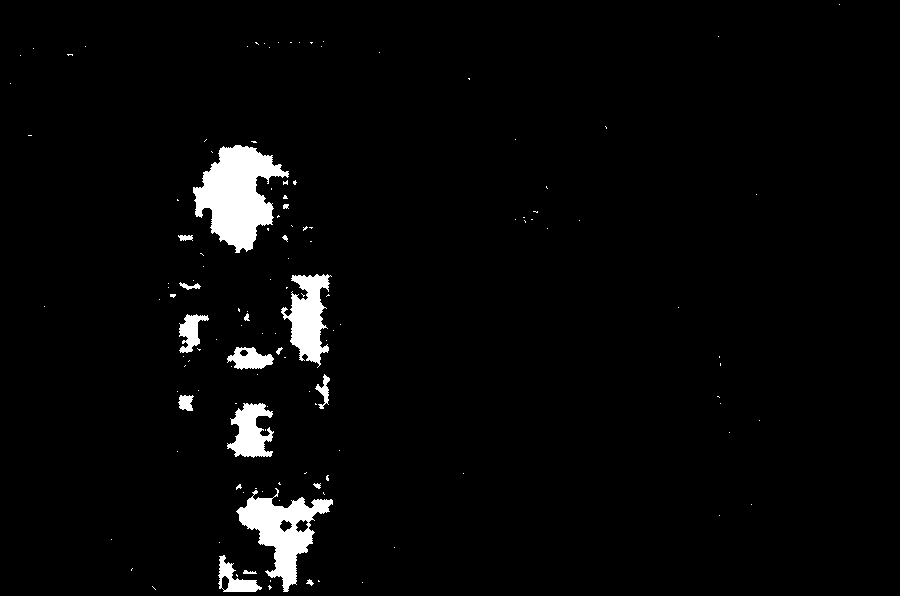
\includegraphics[width=0.95\textwidth]{img/fd2/overSaturated.png}
  \caption{}
\end{subfigure}%

\caption{Original image (a) and the mask of oversaturated regions (b).}
\label{fig:overSaturated}
\end{figure}

Another mask that we construct and detract from the original eye map is one derived from the mean colors of each channel between the pixels inside of the face mask. The mask for this example can be seen in Figure \ref{fig:averageFaceColorMask}, however it does not do provide much benefit in this case. There are though cases when this procedure will remove curls of hair hanging down on the forehead which is why we came to think about this solution. The solution is based on the assumption that we should be able to derive a better mask for the skin of the face after we have derived the face mask and that the eyes should lie inside of the filled version of that skin mask.

\begin{figure}[H]
\centering
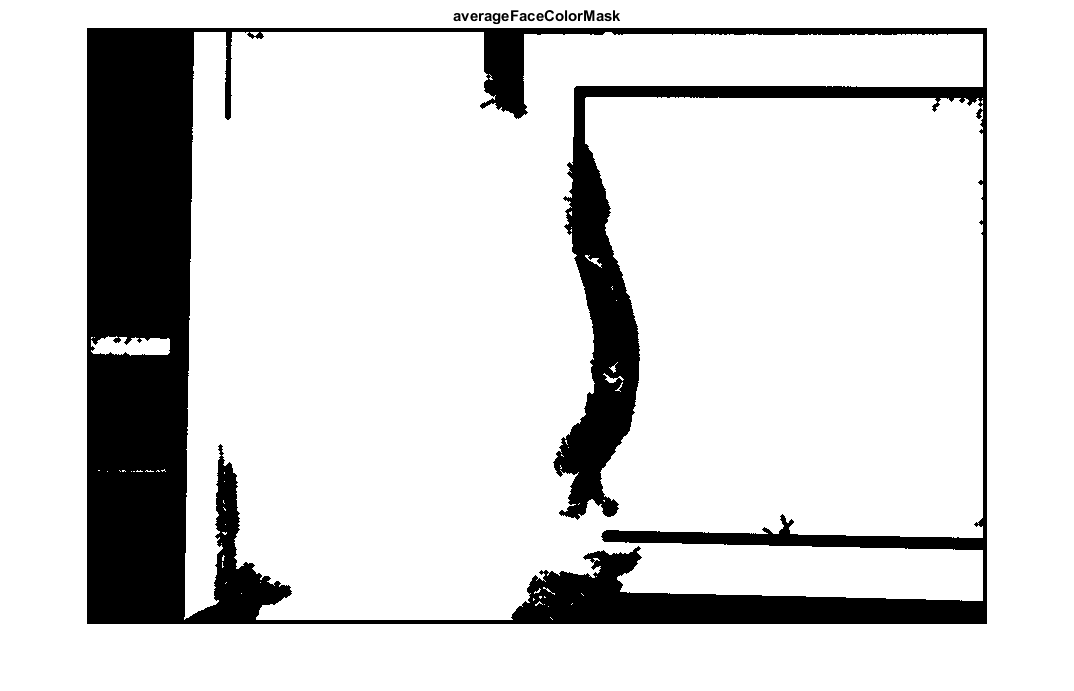
\includegraphics[width=0.3\textwidth]{img/fd2/averageFaceColorMask.png}
\caption{Mask containing the pixels of the original image that lie close to the mean color of the face mask. Here is pixels with a maximum difference of 20 percent from the mean value of each channel allowed. This as we have found that individual comparisons of the values of each channel works better than comparing the actual colors (RGB vectors).}
\label{fig:averageFaceColorMask}
\end{figure}

Finally we also detract a tentative mouth mask and everything outside of the face mask while AND-ing that resulting mask with a dilated version of the mask containing the eye candidates seen in Figure \ref{fig:eyeMap}\textit{e}. This execution gives us the final eye map (depicted in Figure \ref{fig:eyeMap}\textit{f}) that we will hand over to the Hough transform that will try to find the true locations of the eyes.


\subsubsection{Mouth map}

The mouth map seen in Figure \ref{fig:mouthMap}\textit{a} is computed by 
Equation \ref{eq:mouthMap} after the face has been aligned by compensating for the rotations in the image plane. By thresholding the mouth map with half of the maximum value inside of the rectangular mask seen in Figure \ref{fig:mouthMap}\textit{b} we find blobs of mouth candidates. Figure \ref{fig:mouthMap}\textit{b} is derived from the eyes by measuring the distance between them while using this distance when estimating where the mouth should be located. Then by selecting the largest blob among the mouth candidates we determine the mouth mask seen in Figure \ref{fig:mouthMap}\textit{c} and by computing its centroid we also determine its location. 

\begin{figure}[H]
\centering

\begin{subfigure}{.33\textwidth}
  \centering
  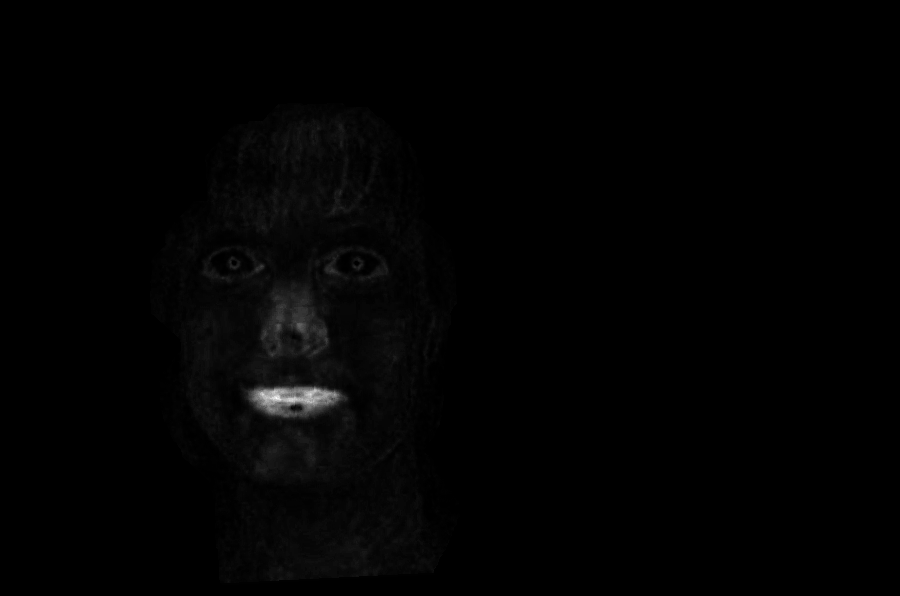
\includegraphics[width=0.95\textwidth]{img/fd/MouthMask.png}
  \caption{}
  % \label{fig:sub1}
\end{subfigure}%
\begin{subfigure}{.33\textwidth}
  \centering
  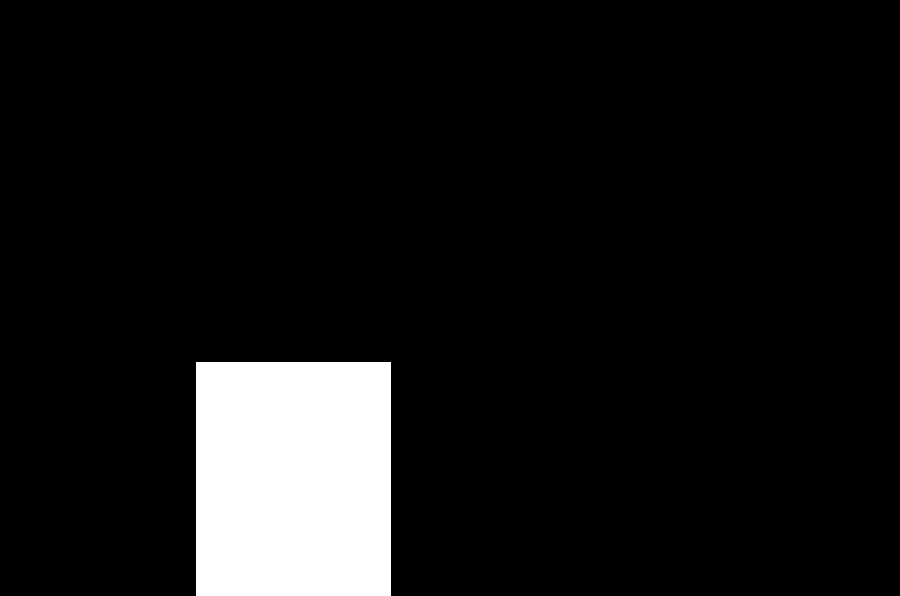
\includegraphics[width=0.95\textwidth]{img/fd/notNonMouthMask.png}
  \caption{}
  % \label{fig:sub1}
\end{subfigure}%
\begin{subfigure}{.33\textwidth}
  \centering
  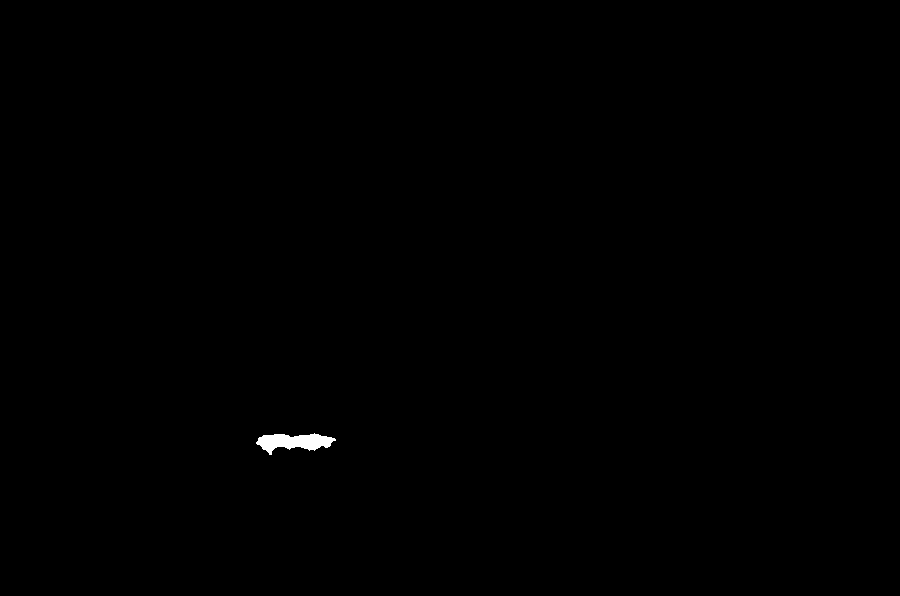
\includegraphics[width=0.95\textwidth]{img/fd/MouthBlob.png}
  \caption{}
  % \label{fig:sub1}
\end{subfigure}%

\caption{Process of computing the location of the mouth. (a) show the mouth map, (b) a mask for the region where the mouth should be located while (c) show the final mouth mask.}
\label{fig:mouthMap}
\end{figure}





\subsubsection{Output}

When the final eye map, Figure \ref{fig:eyeMap}\textit{f}, has been computed we compensate for any rotations less than 90$^{\circ}$ inside of the image plane in order to align the face. We find the rotation of the face by determining the angle of the vector ranging from the left eye to the right eye. Figure \ref{fig:rotationAndOutput}\textit{a} show the face image and the locations of the eyes before the compensating rotation has taken place while Figure \ref{fig:rotationAndOutput}\textit{b} show the compensated image. Finally by measuring the horizontal distance between the eyes and the vertical distance between the eyes and mouth we can derive the output of the face detection phase seen in Figure \ref{fig:rotationAndOutput}\textit{c}.

\begin{figure}[H]
\centering

\begin{subfigure}{.33\textwidth}
  \centering
  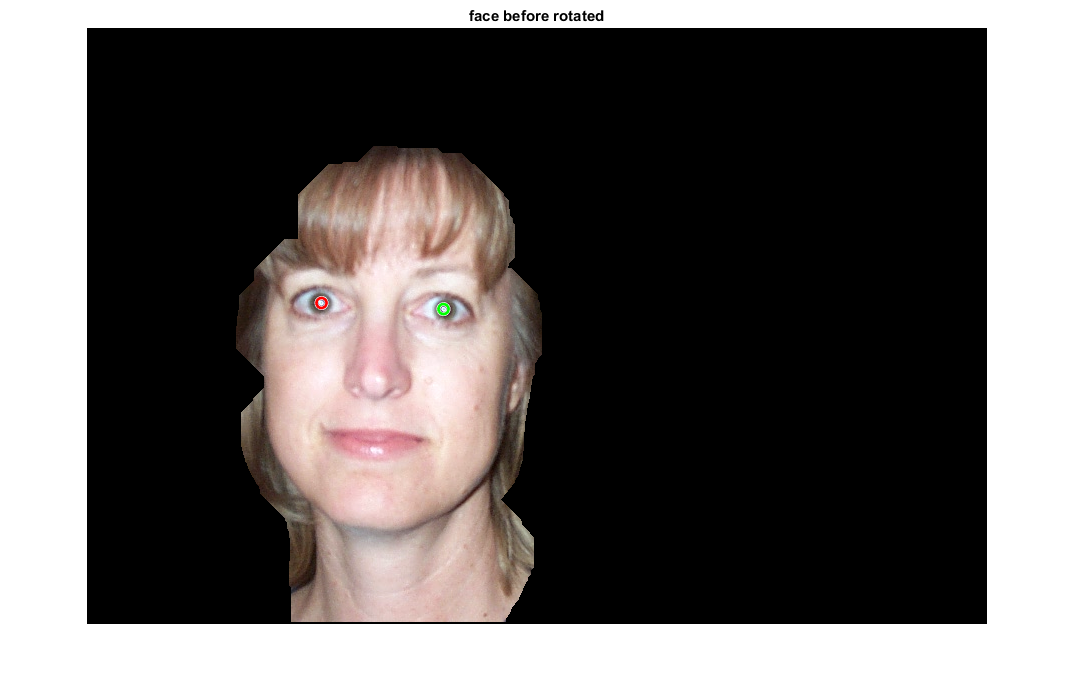
\includegraphics[width=0.95\textwidth]{img/fd2/BeforeRotated.png}
  \caption{}
\end{subfigure}%
\begin{subfigure}{.33\textwidth}
  \centering
  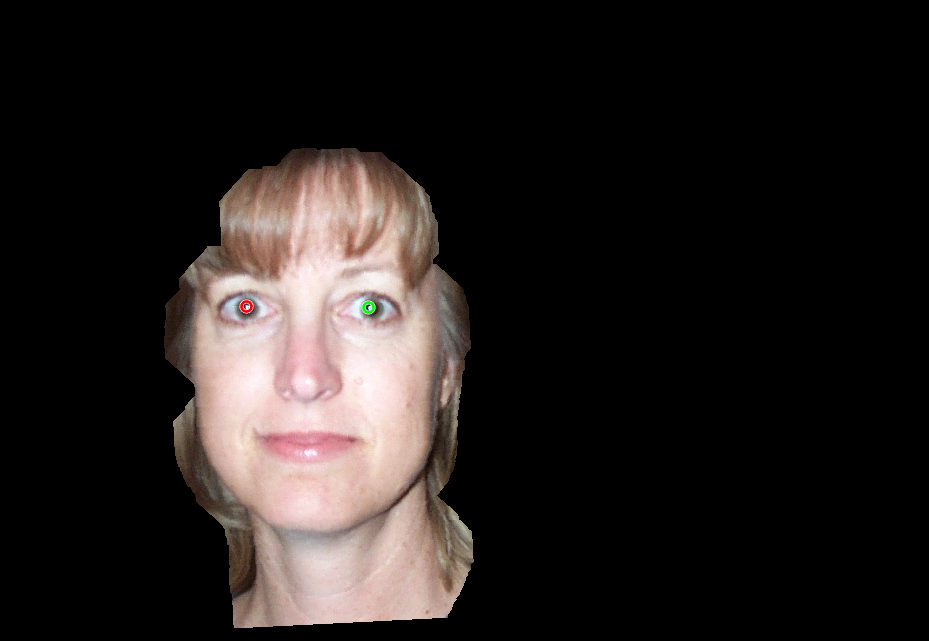
\includegraphics[width=0.95\textwidth]{img/fd2/AfterRotated.png}
  \caption{}
\end{subfigure}%
\begin{subfigure}{.33\textwidth}
  \centering
  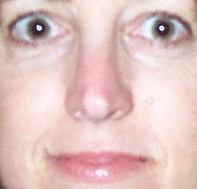
\includegraphics[width=0.6\textwidth]{img/fd2/output12.png}
  \caption{}
\end{subfigure}%

\caption{Aligning the eyes to the horizontal axis. (a) show the face image before correction of the rotation in the image plane is performed, (b) show the rotated version and (c) the final output.}
\label{fig:rotationAndOutput}
\end{figure}


% \begin{figure}[H]
% \centering
% 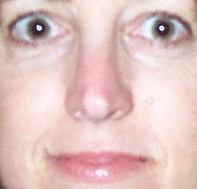
\includegraphics[width=0.16\textwidth]{img/fd2/output12.png}
% \caption{Output of the face detection phase given the input Figure \ref{fig:faceMasks}\textit{a}.}
% \label{fig:fdResult}
% \end{figure}

